%% Type de document et encodage de la police
\documentclass[a4paper]{article}
\usepackage[utf8x]{inputenc}
\usepackage[T1]{fontenc}
% \usepackage[french]{babel}

%% Initialise la taille des pages et des marges
\usepackage[a4paper, top=3cm, bottom=3cm, left=2cm, right=2cm, marginparwidth=2cm]{geometry}

%% Packs utiles
\usepackage{amsmath}
\usepackage{graphicx}
\usepackage{xcolor}

%% Commandes perso
\renewcommand{\arraystretch}{1.2} %% row 20% longer
\definecolor{sprinen}{rgb}{0.0, 1.0, 0.7}

%% Pour les exemples
\usepackage{mdframed}
\newmdenv[topline=false, bottomline=false, rightline=false, skipabove=\topsep, skipbelow=\topsep]{example}

%% Pour les diagrammes
\usepackage{tikz}
\usetikzlibrary{shapes, arrows, calc}
\tikzstyle{incolore} = [rectangle, rounded corners, draw=black, minimum height=1cm, minimum width=3cm, text width=3cm, text centered]


\title{Introduction à la Sécurité Informatique}
\author{Grégoire Roumache}
\date{Décembre 2019}

\begin{document}

\maketitle















\section{Principes de sécurité informatique}





\begin{itemize}





\item \textbf{Système d'information} (SI) = ensemble organisé de ressources qui permet de collecter, stocker, traiter et distribuer de l'information. Composé de 2 sous-systèmes:
\begin{itemize}
    \item sous-système social = structure organisationnelle et des personnes liées au SI
    \item sous-système technique = technologies (hardware, software)
\end{itemize}





\item \textbf{Système informatique} = outil au service du SI.





\item Objectif de la sécurité = réduire les risques et limiter leurs impacts sur le fonctionnement des organisations.





\item Enjeux et impacts de la sécurité des SI:
\begin{itemize}
    \item impacts financiers,
    \item impacts sur l'image et la réputation,
    \item impacts juridiques et réglementaires,
    \item impacts organisationnels.
\end{itemize}





\item Sécurité des SI --- Domaines d'applications:
\begin{itemize}
    \item sécurité du web,
    \item sécurité des données,
    \item sécurité des applications,
    \item sécurité des réseaux,
    \item sécurité du système d'exploitation,
    \item sécurité physique.
\end{itemize}





\item Sûreté v.s. Sécurité --- au-delà du vocabulaire, garder à l'esprit les 2 facettes du danger:
\begin{itemize}
    \item les accidents involontaires,
    \item les actions malveillantes volontaires.
\end{itemize}





\item Le raisonnement de Mr X est le suivant: "comme j’ai, à tout moment, une copie de mon fichier dans le cloud, mon ordinateur est sécurisé". Qu'en pensez-vous ?
\begin{example}
    Faux: l'ordinateur peut toujours être piraté. Et il y a des risques particuliers à utiliser le cloud, ex: l'entreprise qui gère le cloud fait faillite.
\end{example}










\newpage










\item 3 objectifs principaux à ne pas perdre de vue:
\begin{enumerate}
    \item \textbf{Confidentialité}
    \begin{example}
        A et B échangent un message. Ils doivent rester les seuls à en connaître le contenu. \\
        Danger = accès non-désiré à l'information (accidentel ou intentionnel)
    \end{example}
    \item \textbf{Intégrité}
    \begin{example}
        A et B échangent un message. B le reçoit tel que A l'a envoyé (non-modifié). \\
        Danger = altération non-désirée de l'information (accidentelle ou intentionnelle)
    \end{example}
    \item \textbf{Disponibilité}
    \begin{example}
        Les systèmes informatiques doivent rester opérationnels pour permettre l'accès constant à la ressource souhaitée. \\
        Danger = non-disponibilité (accidentelle ou intentionnelle)
    \end{example}
\end{enumerate}





\item Autres objectifs importants --- la triade AAA:
\begin{enumerate} \setcounter{enumi}{3}
    \item \textbf{Authentification}
    \begin{example}
        A et B doivent disposer d’un moyen technique de prouver qui ils sont. \\
        Danger = usurpation d’identité
    \end{example}
    \item \textbf{Autorisation}
    \begin{example}
        A, B et C accèdent à un fichier. C peut le lire, B peut aussi le modifier et A peut également le supprimer. \\
        Danger = accès non-autorisé ou accès avec de mauvaises autorisations
    \end{example}
    \item \textbf{Accounting} (= journalisation/auditabilité)
    \begin{example}
        Le système doit fournir un outil permettant de dire qui fait quoi. \\
        Danger = incapacité de déterminer qui ou comment on utilise les ressources du SI \\
        Remarque: \textbf{Attention} au lien étroit entre cet objectif et la loi (tracker les utilisateurs...).
    \end{example}
\end{enumerate}





\item Derniers objectifs:
\begin{enumerate} \setcounter{enumi}{6}
    \item \textbf{Autenticité}
    \begin{example}
        A envoie un message à B. B doit avoir une preuve que c'est bien A qui l'a envoyé.
    \end{example}
    \item \textbf{Non-répudiation} (irrévocabilité)
    \begin{example}
        Empêcher une entité (personne, entreprise) de nier une action accomplie. \\
        Danger = nier volontairement des actions accomplies ou des engagements pris.
    \end{example}
\end{enumerate}





\item Authentification v.s. Identification
\begin{itemize}
    \item Identification = répondre à la question: "qui êtes vous ?".
    \item Authentification = en apporter la preuve.
\end{itemize}





\item Causes de l'évolution des risques:
\begin{itemize}
    \item multiplication des systèmes d'informations,
    \item démocratisation des outils informatiques,
    \item généralisation des accès à Internet,
    \item complexité des architectures,
    \item diversification de la nature des données,
    \item professionnalisations des acteurs malveillants, ...
\end{itemize}





\item Motivations des attaques:
\begin{itemize}
    \item raisons politiques,
    \item idéologiques,
    \item financières,
    \item ludiques, ...
\end{itemize}





\item \textbf{Vulnérabilité} = faiblesse au niveau d’un bien (au niveau de la conception, réalisation, installation, configuration, utilisation).





\item \textbf{Menace} = cause potentielle d’un incident.





\item \textbf{Risque} = menace $ \times $ vulnérabilité





\item Criticité = probabilité du risque $ \times $ impacts (= $ P_{risque} \times impacts $) \\
Remarque: la priorité est mise sur les mesures qui préviennent les événements les plus critiques.





\item \textbf{Attaque} = action malveillante destinée à porter atteinte à la sécurité d’un bien. C'est la concrétisation d’une menace, elle exploite une vulnérabilité.





\item \textbf{Qui fait quoi ?}
\begin{itemize}
    \item Black Hats = hacker malintentionné
    \item Grey Hats = hacker parfois éthique et parfois pas
    \item White Hats = hacker éthique
    \item Script Kiddies = hacker inexpérimenté, utilise des programmes/scripts développés par d'autres
    \item Cyber terroriste = personne détruisant de manière systématique des systèmes informatiques pour atteindre un but politique grâce à la menace ou l'intimidation
    \item Hacktiviste = piratage informatique dans le but de favoriser des changements politiques ou sociétaux
    \item Crackers = hacker qui casse des protections de sécurité (ex: logiciel avec clé d'enregistrement)
    \item Carder = hacker qui pirate des cartes de crédit
    \item Phreaker = personne exploitant frauduleusement les systèmes téléphoniques
    \item \textbf{RSSI} = Responsable de la Sécurité des Systèmes d'Information
\end{itemize}





\item Méthodologie du hacker:
\begin{enumerate}
    \item collecte de l’information
    \item intrusion
    \item (option) garantir un accès plus facile dans le futur
    \item reconnaissance interne
    \item (option) mouvement
    \item exécution de l’action voulue
    \item (option) couvrir les traces
\end{enumerate}





\item Différents types d'attaques:
\begin{itemize}
    \item Virus = programme malveillant qui se réplique et modifie des données/programmes
    \item Ver = programme malveillant qui se réplique (sans modifier les données/programmes)
    \item Cheval de Troie = programme malveillant caché à l'intérieur d’un programme à l'allure légitime
    \item Spyware = logiciel "espion", récolte des informations sur le système ou l'utilisateur
    \item Adware = force l'utilisateur à regarder des pubs ou se rend sur des sites pour générer des revenus publicitaires
    \item Spam (pourriel) = messages envoyés à des fins publicitaires ou malveillantes
    \item Ransomware = chiffre les données sur l'ordinateur et demande une rançon pour les déchiffrer
    \item Phishing = site se faisant passer pour un site web authentique pour voler des données de connexion
    \item DoS - DDoS = empêche ou limite fortement la capacité d’un système à fournir le service attendu
    \item MitM (man in the middle) = interception des échanges entre 2 parties légitimes
\end{itemize}





\end{itemize}















\section{Guide d’hygiène informatique}





\begin{itemize}





\item Citer une technique permettant le cloisonnement des réseaux.
\begin{example}
    VLAN, switch, firewall, cloisonnement physique (= séparation physique)
\end{example}





\item À qui est destiné une charte informatique ?
\begin{example}
    Destinée aux utilisateurs des systèmes informatiques, généralement mise à disposition des employés par l'employeur. \\
    Dans le cas de l'hénallux, elle est signée par les représentants syndicaux (des profs et de l'administration) et la direction mais pas par une organisation représentant les étudiants.
\end{example}





\item Journalisation:
\begin{itemize}
    \item De quoi s'agit-il ?
    \begin{example}
        C'est l'enregistrement séquentiel dans un fichier ou une base de données de tous les événements affectant un processus particulier (application, activité d'un réseau informatique…).
    \end{example}
    \item Comment rendre son utilisation optimal ?
    \begin{example}
        Tout enregistrer (toutes les applications ouvertes et quelles actions l'utilisateur prend, etc.).
    \end{example}
    \item Quelle est la différence avec le monitoring ?
    \begin{example}
        monitoring = surveillance/mesure d'une activité informatique en temps réel (ex: mesurer les performances)

        Autrement dit,
        \begin{itemize}
            \item monitoring = analyse en temps réel
            \item journalisation = enregistrement pour analyse plus tard
        \end{itemize}
    \end{example}
\end{itemize}





\item \textbf{Définition}:
\begin{itemize}
    \item RSSI = Responsable de la Sécurité des Systèmes d'Information
    \item Infogérant = prestataire \textbf{externe} de gestion ou d'exploitation d'un système informatique
    \item Risques SSI = Risques de Sécurité des Systèmes d'Information
    \item Hébergement mutualisé = serveurs informatiques dont les ressources sont attribuées dynamiquement à un ensemble d'utilisateurs
    \item Appel d’offre = procédure permettant à un commanditaire de faire le choix de l'entreprise la plus à même de réaliser une prestation de travaux, fournitures ou services. Le but est de mettre plusieurs entreprises en concurrence.
\end{itemize}





\item Notion intéressante: plan d’assurance sécurité PAS.
\begin{example}
    Remarque: PAS = Plan d'Assurance Sécurité. \\
    Le PAS a pour but de préciser comment les prestataires se conforment aux exigences de cybersécurité définies par le maître d’ouvrage.
\end{example}





\item Relais applicatifs
\begin{itemize}
    \item Autre terme pour \textit{relai applicatif}.
    \begin{example}
        Proxy (= logiciel intermédiaire en se plaçant entre deux hôtes pour faciliter ou surveiller leurs échanges)
    \end{example}
    \item Protocole les utilisant fréquemment.
    \begin{example}
        HTTP (plus généralement, couche application: http, ssh, ftp, etc.)
    \end{example}
\end{itemize}





\item De quoi découlent les politiques de sécurité ?
\begin{example}
    politiques de sécurité = plan d'actions définies pour maintenir un certain niveau de sécurité \\
    Elle découle de la stratégie de l'entreprise \textcolor{red}{\textbf{(??)}}
\end{example}





\item Que veut dire "les procédures doivent être formalisées" ?
\begin{example}
    Les procédures doivent être précises, nettes et exclure tout malentendu. \\
    Remarque: procédure = manière spécifiée d'effectuer un ensemble de tâches.
\end{example}





\item Comptes services, utilisateurs et d’administration:
\begin{itemize}
    \item Quelle est la nomenclature pour identifier les comptes ?
    \begin{example}
        "il est souhaitable de définir et d’utiliser une nomenclature simple et claire pour identifier les comptes de services et les comptes d’administration"
    \end{example}
    \item Donner un exemple (logiciel = Tech3d, utilisateur = Céline Heliot, admin IT = Louis Renard).
    \begin{example}
        Noms des comptes:
        \begin{itemize}
            \item Céline Heliot = user-celine-heliot
            \item Louis Renard = admin-louis-renard
        \end{itemize}
        Objectifs = connaître directement les droits des comptes àpd leurs noms.
    \end{example}
\end{itemize}





\item \textbf{Définitions}:
\begin{itemize}
    \item SSID Wi-Fi = nom du wifi
    \item 802.1X = protocole d'identification wifi avec nom d'utilisateur et mot de passe (comme à l'hénallux)
\end{itemize}





\item Condensat de mot de passe:
\begin{itemize}
    \item Autre terme plus utilisé.
    \begin{example}
        hash
    \end{example}
    \item Est-ce robuste ?
    \begin{example}
        oui, si on utilise une bonne fonction de hashage
    \end{example}
\end{itemize}





\item Authentification:
\begin{itemize}
    \item Pourquoi une authentification à 2 facteurs est plus robuste ?
    \begin{example}
        Car plus difficile de voler deux facteurs qu'un seul.
    \end{example}
    \item Authentification multi-facteurs:
    \begin{itemize}
        \item Quelque chose que je sais,
        \item Quelque chose que je possède,
        \item Quelque chose que je suis.
    \end{itemize}
    \item Le dernier facteur d'authentification (ce que je suis) est-il une bonne idée ?
    \begin{example}
        Non. Une fois que ce facteur est compromis, il est difficile à changer, vu qu'on ne peut pas se changer soit même.
    \end{example}
    \item Qu’est-ce qu’une carte RFID ?
    \begin{example}
        Une carte de radio-identification.
    \end{example}
    \item Donner un exemple de "Mécanisme de mots de passe à usage unique avec jeton physique".
    \begin{example}
        Lorsqu'on utilise le PC banking, le lecteur de carte créé un mot de passe à usage unique.
    \end{example}
\end{itemize}





\item Qu’est-ce qu’une application ou un serveur métier ?
\begin{example}
    Une application métier sert à gérer l'activité de l'entreprise. L'application est existante ou développée selon les besoins métiers.
\end{example}





\item Pourquoi le \textit{backup} doit se faire sur des équipements déconnectés ?
\begin{example}
    Si ils sont connectés, ils sont vulnérables et on perd l'avantage de faire un backup.
\end{example}





\item À quoi correspondent les ports que le document recommande de bloquer:
\begin{itemize}
    \item 135, 445 et 3389 pour Windows,
    \item 22 pour Linux ?
\end{itemize}
\begin{example}
    Ce sont les ports qui permettent de prendre le contrôle à distance de l'ordinateur.
\end{example}





\item "les infrastructures d’hébergement Internet doivent être physiquement cloisonnées de toutes les infrastructures du système d’information qui n’ont pas vocation à être visibles depuis Internet" \\
Quelle technique se cache derrière cette recommandation ?
\begin{example}
    Le pare-feu (firewall).
\end{example}
\begin{center}
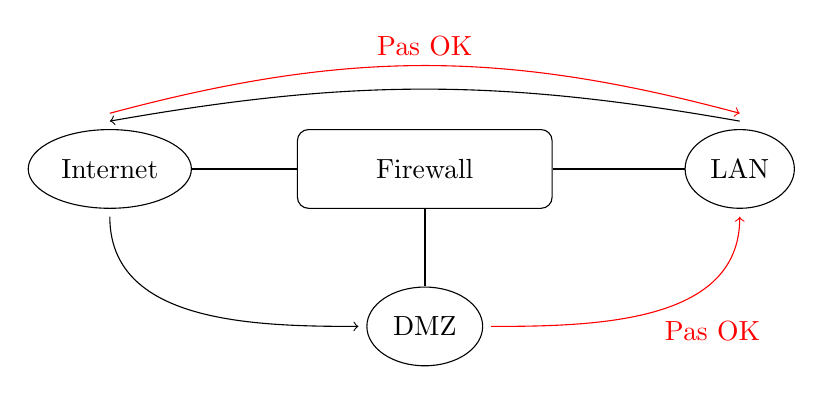
\begin{tikzpicture}
    \node (firewall) [incolore] {Firewall};
    \node (internet) [ellipse, draw=black, minimum width=2.5, minimum height=1cm] at (-4,0) {Internet};
    \node (lan) [ellipse, draw=black, minimum width=2.5, minimum height=1cm] at (4,0) {LAN};
    \node (dmz) [ellipse, draw=black, minimum width=2.5, minimum height=1cm] at (0,-2) {DMZ};

    \draw[thick] (internet) -- (firewall);
    \draw[thick] (lan) -- (firewall);
    \draw[thick] (dmz) -- (firewall);

    \draw [<-] ($(internet.north) + (0,0.1)$) to [out=10, in=170] ($(lan.north) + (0,0.1)$);
    \draw [->, red] ($(internet.north) + (0,0.2)$) to [out=15, in=165] node[anchor=south]{Pas OK} ($(lan.north) + (0,0.2)$);

    \draw [->] ($(internet.south) + (0,-0.1)$) to [out=-90, in=-180] ($(dmz.west) + (-0.1,0)$);
    \draw [<-, red] ($(lan.south) + (0,-0.1)$) to [out=-90, in=0] node[anchor=north west]{Pas OK} ($(dmz.east) + (0.1,0)$);
\end{tikzpicture}
\end{center}
Remarque: DMZ = zone démilitarisée, peut contenir des serveurs web, ftp, smtp.





\item Qu’est-ce qu’un tunnel « site à site » ? Sur quel appareil monter un tel tunnel ?
\begin{example}
    C'est un tunnel VPN qui sert à communiquer de manière sécurisée sur internet. On monte ce tunnel sur des routeurs.
\end{example}
\begin{center}
\begin{tikzpicture}
    \node (r1) [anchor=west] at (-4,0) {\includegraphics[width=1cm]{images/router.jpg}};
    \node (r2) [anchor=east] at (4,0) {\includegraphics[width=1cm]{images/router.jpg}};

    \node [ellipse, draw=black, minimum width=2.5, minimum height=1cm, anchor=east] at (-3.8,0) {LAN BXL};
    \node [ellipse, draw=black, minimum width=2.5, minimum height=1cm, anchor=west] at (3.8,0) {LAN Namur};

    \draw ($(r1) + (0,0.05)$) -- ($(r2) + (0,0.05)$);
    \draw ($(r1) + (0,-0.05)$) -- ($(r2) + (0,-0.05)$);

    \node [ellipse, draw=black, anchor=west, minimum height=2.5cm, minimum width=5.5cm] at ($(r1.east) + (0,-0.3)$) {Internet};
\end{tikzpicture}
\end{center}










\newpage










\item Qu’est-ce qu’un serveur mandataire inverse ?
\begin{example}
    serveur mandataire inverse = reverse proxy
    \begin{itemize}
        \item proxy = serveur permettant à un utilisateur d'accéder à internet
        \item reverse proxy = serveur permettant à un utilisateur d'internet d'accéder à des ressources internes
    \end{itemize}
\end{example}





\item Que sont les enregistrements DNS: MX, SPF, DKIM, DMARC ?
\begin{example}
    Des enregistrements mails (ex: MX = mail exchanger record).
\end{example}





\item Quels outils pour la délégation de privilèges ?
\begin{example}
    \textcolor{red}{\textbf{(??)}}
\end{example}





\item Quel est le risque de chiffrer ses données ?
\begin{example}
    De perdre la clé de déchiffrement.
\end{example}





\item \textbf{Définitions}:
\begin{itemize}
    \item Adhérence logicielle = interdépendance entre programmes qui ont besoin les uns des autres pour fonctionner
    \item Corrélation = lien, rapport réciproque
    \item Protocole NTP = Network Time Protocol
    \item EBIOS = méthode d'analyse de risque de l'ANSSI
\end{itemize}





\end{itemize}










\end{document}
